\documentclass[oneside,12pt,a4paper,final]{book}
%\usepackage[margin=3cm]{geometry}
\usepackage[utf8]{inputenc}
\usepackage{amsmath}
\usepackage{amsfonts}
\usepackage{amssymb}
\usepackage{graphicx}
\usepackage{setspace}
\usepackage{arabtex}
\usepackage{utf8}
\newcommand{\HRule}{\rule{\linewidth}{0.6mm}}
%\usepackage{hyperref}
\usepackage{listings}
\lstset{language=C}
\usepackage[acronym]{glossaries} 
\makeglossaries
\author{Nacer Khalil}
\title{Internet of Things: a Real-World Deployment Towards Smart Grids Integration}

\newenvironment{dedication}{\vspace{6ex}\begin{quotation}\begin{center}\begin{em}}{\par\end{em}\end{center}\end{quotation}}

    
\begin{document}
\doublespacing
\newacronym{ipv4}{IPV4}{Internet protocol version 4}
\newacronym{ipv6}{IPV6}{Internet protocol version 6}
\newacronym{iot}{IOT}{Internet of things}
\newacronym{j2se}{J2SE}{Java Standard edition}
\newacronym{tinyos}{TinyOS}{TinyOS}
\newacronym{nesc}{NesC}{NesC}
\newacronym{http}{HTTP}{Hypertext Transfer protocol}


\frontmatter

%COVER PAGE
\begin{titlepage}
\begin{center}

\includegraphics[width=0.6\textwidth]{img/aui_logo.jpg}
%
\includegraphics[width=0.45\textwidth]{img/tum_logo.jpg}
\linebreak
\linebreak
\linebreak
% Title
\HRule \\[0.4cm]
{ \huge \bfseries Internet of Things: a Real-World Deployment Towards Smart Grids Integration}\\[0.4cm]

\HRule \\[1.5cm]

% Author and supervisor
\begin{minipage}{0.4\textwidth}
\begin{flushleft} \large
\emph{Author:}\\
Nacer \textsc{Khalil}
\end{flushleft}
\end{minipage}
\begin{minipage}{0.4\textwidth}
\begin{flushright} \large
\emph{Supervisor:} \\
Dr.~Mohamed Riduan \textsc{Abid} \\
Dr.~Driss \textsc{Benhaddou} \\
Dr.~Michael \textsc{Gerndt} 
\end{flushright}
\end{minipage}

\vfill

% Bottom of the page
{\large \today}

\end{center}
\end{titlepage}

\chapter{} % dedications chapter
\begin{dedication}
To my dear parents for their patience, love and support \\
To my brothers Hossein, Omar and Saad \\
To my cousin Sara and her family \\
To my family \\
To my friends \\

\end{dedication}
\chapter{Acknowledgments}
\paragraph{}
I am deeply thankful to my supervisor Dr. Mohamed Riduan Abid for his very close supervision, guidance and for the advice he kept giving me during the lifetime of the project. Your advices whether they are computer science related, or even every day life related wise words things I will never forget.
\paragraph*{}
I am also thankful for having Dr. Driss Benhaddou as a supervisor. His advice, insight, guidance and very enlightening ideas. I wouldn't have been so interested in smart grids without the discussions we had on the topic.
\paragraph{}
I would also like to thank Dr. Michael Gerndt for his guidance in this thesis and also for his help and advising throughout my masters degree in Technische Universät München.
\paragraph{}
I  also thank Dr. Hamid Harroud who suggested several directions to take throughout the course of this project.
\paragraph{}
My special thanks to my close friends who helped relax in times that seemed very stressful. I wouldn't have made it without their help.
\paragraph{}
I also greatly thank all excellent professors of whom I had the chance to be a student. I learned things in class  I would have never learnt elsewhere.


\chapter{Abstract}
\paragraph{}
The Information Technology is advancing exponentially and largely bigger impacting our daily lives. The current evolution in computing is called the \gls{iot}. It is smoothly evolving from an Internet of people to and Internet of Things. By 2020, it is expected to have 50 billion "Things" connected to the Internet. 
\paragraph{}
However such a migration induces a strong level of complexity when handling interoperability between heterogeneous things, i.e. Wireless Sensors, RFID, and mobile computing.
\paragraph{}
In this thesis, we focus on the  integration of wireless sensors into \gls{iot}. This prologues for a future integration of \gls{sg}\glsreset{sg} into \gls{iot}. In this work, we deployed a smart building testbed for energy optimization.
\paragraph{}
The system is using different technologies such as \gls{tinyos}, \gls{nesc}, \gls{j2se} and  \gls{http}.

\chapter{Résumé}
\paragraph{}
La technologie de l'information progresse de façon exponentielle et prend largement plus impact sur nos vies quotidiennes. L'évolution actuelle de l'informatique est appelé \glsreset{iot}\gls{iot}. il est prévu d'avoir en 2020 50 milliards "choses" connecté à l'Internet.
\paragraph{}
Cependant, une telle migration induit un fort niveau de complexité lorsque l'interopérabilité entre en jeu entre differentes choses hétérogènes, à savoir capteurs sans fil, RFID et l'informatique mobile.
\paragraph{}
Dans cette thèse, nous nous concentrons sur l'intégration de capteurs sans fil dans \gls{iot}. Cela conduit vers une future intégration de Smart Grid (SG) dans \gls{iot}. Au cours de ce projet, nous avons déployé un banc d'essai intelligente du bâtiment pour l'optimisation de l'énergie.
\paragraph{}
Ce système d'information utilise différentes technologies  telles que TinyOS (TinyOS), \glsreset{nesc}\gls{nesc}, Java Standard Edition (J2SE), HTTP.


\setcode{utf8}

%\chapter{ملخص}

\chapter{Arabic}
\paragraph{}
\begin{arabtex}
تكنولوجيا المعلومات تتقدم باطراد وجود أكبر تأثير على حياتنا كما تقدم الوقت. الثورة القادمة في مجال الحوسبة يسمى إنترنت الأشياء (قام المحفل). انها اساسا شبكة الانترنت ونحن نعلم في الوقت الحاضر إلا أن الأشياء المادية (ثلاجة، تلفزيون، تكييف هواء ...) وسوف تكون القوى الفاعلة الرئيسية في هذا النظام المعقد. وفي هذا السياق، فإن المشروع يبني على هذه الفكرة على سرير اختبار لترشيد استهلاك الطاقة الذكية الرئيسية. ال يسمح المشروع للمستخدمين لرصد استهلاك الطاقة لديها عبر الذكية الخاصة بهم الهاتف وأيضا يمكن للمستخدمين التحكم في الأجهزة عن طريق تشغيل وإيقاف الأجهزة عن بعد.
\end{arabtex}
\paragraph{}
\begin{arabtex}
وينقسم النظام إلى ثلاثة عناصر رئيسية. كل واحد منهم يستخدم
التكنولوجيات المختلفة، مث لTinyOS، NESC، ومعيار جافا
طبعة J2SE، بروتوكول نقل النص التشعبي HTTP وغيرها من التكنولوجيات
التي سيتم مناقشتها في التقرير أطروحة.
\end{arabtex}
\paragraph{}
\begin{arabtex}

في هذه المرحلة، ونظام مراقبة يسمح، ولكن تشغيل وإيقاف تطبيق صحيفة-
 ليس هناك حتى الآن وذلك أساسا بسبب غياب المعدات ولكن البلاغ لهذا الغرض هناك.
\end{arabtex}

\singlespacing

\tableofcontents
\listoffigures
\listoftables
\printglossaries

\mainmatter
\doublespacing
\chapter{Introduction}

\section{Importance of Study}
\paragraph{}
The global electrical grid one the bases that gives us this quality of life that most people around the world enjoy. The global electrical grid is sometimes called the largest machine ever made by man. \cite{ref1}. It a widespread machine, distributed but interconnected system that provides power to households, companies and other organizations and therefore the world's economy is counting on it. The electrical grid knows numerous problems such as blackouts, current instabilities that costs billions of dollars yearly to both the utilities, utilities and insurances. The grid suffers from the problem of peak hours where energy consumption where in many case the one single utility cannot provide such energy.
\paragraph{}
The \gls{sg} comes to provide solutions to the problems that suffers from the traditional electrical grid. \gls{sg} is an intelligent, auto-balancing, and self-monitoring electrical grid \cite{ref2} and is and whose energy sources are distributed between utilities and consumers. The nature of the \gls{sg} as having distributed energy sources reduces numerous losses that arises in the traditional grid such as the energy loss in the energy transmission lines and also in the overload of the electrical lines.
\paragraph{}
Another revolution is about to begin and it is taking place in the information technology and is called \glsreset{iot}\gls{iot}. \gls{iot} is the era of autonomous machine able to produce and consume information and being able to act autonomously without the guidance of humans to performs their tasks. Cisco predicts that the number of devices to be connected in 2020 will break the 50 billions devices \cite{ref3} whereas the world population will be around 7.6 billion. That make 6.58 devices connected for each person in the world whereas the number of devices connected in 2010 12.5 billion. This clearly shows that the shift to the \gls{iot} has already started.
\paragraph{}
\glsreset{sg}\gls{sg} can and will benefit from the \gls{iot}. The integration of the \gls{sg} and and \gls{iot} makes this study and thesis of high importance in order to solve as much as possible the problems of the traditional grid but at the same bring a new dimension to the power grid by benefiting from the numerous possibilities offered by the \gls{iot}.

\section{Rationale of Study}
\paragraph{}
This project has been done in order to investigate ways the \gls{iot} can benefit the \gls{sg}. The smart grid as a set of philosophical ideas counts on a set of novel functionalities. Once of these ideas is the two-way communication that will make possible the utility to communicate with consumers and vice versa. This concept is possible with the Internet Of Things as devices in \gls{iot} communicate between them by producing and consuming information. Numerous ideas are based on this two-way communication such as the \gls{dr} which offers a set of services for both the power provider and the consumer.
\paragraph{}
The \glsreset{iot}\gls{iot} counts on different technologies such as \gls{wsn}, \gls{rfid}, \gls{ipv6} and other technologies which make the Internet of things a very heterogeneous and complex system \cite{ref4}. One of the challenges in \gls{iot} is to deals with such heterogeneity and take the most out of it in order to make the communication as smooth and robust as possible. This heterogeneity should be made transparent to any two parties trying to communicate in \gls{iot}.

\section{Problem Statement}
\paragraph{}
The \glsreset{sg} \gls{sg} counts on the two-way communication to build to a whole communication and protocol stack namely the \glsreset{dr}\gls{dr} and other services built on top of the \gls{dr}. From the consumer's side or more precisely the household's side, there are smart home energy management software in the market nowadays but none of these products offers integration with \gls{sg}. To have such an integration with \gls{sg}, there is a need to first build this two-way communication and make it possible for any appliance to report its real-time energy consumption and also to be able to be controlled remotely with this two-way communication. Such infrastructure is missing for the time being and therefore the integration of the smart home within the smart grid is not possible. Also, in order for \gls{sg} to be integrated into the \gls{iot}, all devices should be able to communicate in the two directions.
\paragraph{}
As \gls{sg} counts on numerous technologies to achieve its main goals. This usage of different technologies imposes another problem which is the heterogeneity of the system. As numerous components count on different technologies, there is a need to interface them in order to make this heterogeneity transparent to the all components of the system. This means that there is a need to build a software within the whole system that would constitute an important part of it and will take care of making the communication and processes technology-transparent and give the possibility to all components of the system to work hand-in-hand in order their common goals independently of the data link layer technology (Ethernet, Wifi or Zigbee) they are counting on, the network layer technology (\gls{ipv4} or \gls{ipv6}).

\section{Purpose of Study}
 \paragraph{}
The goal of the study is to solve the problems introduced in the problem statement section. This means creating the two-way communication, and also solving the heterogeneity that arises from integrating smart homes with the smart grid and making each components in the smart home as part of the Internet of things by making it communicate with any device in the Internet and having an \gls{ipv6} address that is built by making use of \gls{6lowpan} whose goal is to provide the TCP/IP to the smallest devices and with the least computational and energy rich.
\paragraph{}
The first purpose of this study is to create a testbed having the two-way communication and also being able to make use of it in order to build richer applications based on this possibility. To do it, there was a need to first introduce \gls{6lowpan} within every device in the \gls{wsn}. This would make every sensor node also known as mote identified and ready to communicate and be part of the \gls{iot}. This communication will go in the two directions and based on that the two-way communication will have to be built.
\paragraph{}
The second purpose of this study is to solve the heterogeneity problem that arises with the integration of smart homes within the smart grid and also when making the whole system as part of the \glsreset{iot}\gls{iot}. Solving such a problem means having an additional component that will track all communication packets and change them to fit the needs of the destination component. This will make of this additional component a middleman and therefore make the heterogeneity problem disappear.

\section{Scope of Study}
\paragraph{}
The thesis aims to solves the two problems presented in section 1.3. To do so, a variety of tools and technologies were used for this purpose.The two problems were not solved one independently of the other but even though the problems seem separate one cannot solve without having to solve the other. In other words, after the creation of the two-way communication in the \glsreset{wsn}\gls{wsn} which supported \gls{ipv6} over \gls{6lowpan}, other network only supported \gls{ipv4} and therefore could not communicate, and this was due to the heterogeneity problem. This is why the two-way communication was created and then the heterogeneity problem had to be solved in order to see everything working.
The system is divided into four components:
\begin{itemize}
\item The fully \gls{ipv6} supported \gls{wsn}
\item The \gls{tinyos} program for sensor transmission and appliance request handler
\item The heterogeneity handler and middleman gateway server
\item The mobile client
\end{itemize}
\paragraph{}
Each of these four component exist to solve part of the problem. Each of these components will be discussed extensively in the Chapter 4 from the architectural aspect of the component and in Chapter 5 from the implementation level of the system. 
\paragraph{}
It is to be noted that some of the concepts will be discussed from the architectural point in Chapter 4 but not from an implementation point in Chapter 5. The sole reason behind is the fact that some of the equipment required for this thesis did not arrive on time and therefore the parts in the implementation requiring such equipment was omitted to meet the deadlines.
\section{Outcome of the Study}
\paragraph{}
The outcome of the thesis is to design and implement a test-bed that is able to show the two-way communication in action. It will also have to show concepts of the \glsreset{iot}\gls{iot} which are that every node in the system can communicate autonomously and with any other node in the Internet. Another \gls{iot} concept is the ability of any node in the \gls{iot} to consume and produce information that is communicated through the network.
\paragraph{}
The autonomous production of information is shown by the fact that every sensor node in the \gls{wsn} reads sensory data from its sensors that are attached to appliance in order to sense their consumption and this information is produced and transmitted periodically. The consumption of data by is shown by external nodes in the \gls{iot} sending request to the sensor node in the \gls{wsn} in order to control and appliance's status i.e. turn on the television. This will prove the consumption of information by the nodes in the \gls{iot}.
\paragraph{}
The test-bed should also show that communication between any two nodes in the \gls{iot} is successful, robust and reliable and that the heterogeneity of the system is made transparent to the nodes in the system by the creation of the software tool residing in the gateway which is between the \gls{iot} and the outside world. This software tool is seen as a heterogeneity handler and also a communication middleman that translates the communication to the appropriate technology needed by the recipient.
\paragraph{}
The testbed will able to show the two-way communication in action and will also show that the heterogeneity does not form a barrier by its successful handling.

\section{Outline of the Thesis}
\paragraph{}
The thesis is is divided into eight chapters. Each of the chapter approaches thesis from a different aspect. 
\paragraph{Chapter 1}
It is an introductory chapter that gives a flavor of the project that is to be studied in this thesis and also introduces the problem and the solution proposed in this topic. This chapter also puts the reader into perspective by introducing some of the main concepts related to the \glsreset{sg}\gls{sg} and the \glsreset{iot}\gls{iot}. 
\paragraph{Chapter 2}
It presents the background of the work by revising the literature related to the topics of \gls{iot} and \gls{sg}. It also discussed related work and how it was tackled in different research papers, how does it relate to the work done in this thesis and also how does it differ.
\paragraph{Chapter 3}
It is dedicated to the \glsreset{iot}\gls{iot}. It presents the topic, talks about the importance of \gls{iot}, its impact on the world, the actual Internet, the future of Internet and also how will \gls{sg} benefit from it.
\paragraph{Chapter 4}
It will present the architecture of the system and the test-bed. It will discuss the system from different aspects, and how were the two problems solved from the architectural aspect.
\paragraph{Chapter 5}
This chapter will mostly discuss the implementation system. It will start by presenting the hardware used in this project, then move to the technology enablers. Each component of the system will be discussed extensively and move to the integration of the components to form the test-bed.
\paragraph{Chapter 6}
It will start first by presenting the findings then move to explain the experiment that was done to measure the performance of the system. The data gathering section will show how and what data was gathered and then move to analyzing and interpreting the data.
\paragraph{Chapter 7, 8}
These are the last two chapters of the thesis that will conclude the thesis, provide directions about future work and recommendations to the reader what parts of the system could be ameliorated and how it can be achieved.
\chapter{Literature Review}
\section{The need for Smart Grid}
\paragraph{}
The actual electrical grid is based on a technology that is at least one century old \cite{ref5}. As a result, there is a need to change as to meet to 21st century requirement such as having more green energy in order to reduce the pollution caused mainly by the use of fossil energy. As a result, research has introduced a new technology called \glsreset{sg}\gls{sg}. Although it is still a research project and numerous issues related to \gls{sg} are left unanswered, nations across the globe started to deploy \gls{sg} project. It is also noted that in order for the grid to become more reliable, secure and efficient, a bi-directional information and communication infrastructure should be embedded within the grid \cite{ref5}.
\paragraph{}
The smart grid brings around new concepts that will achieve efficiency, reliable and security to the power grid. The first one is the introduction of the \gls{dg} by exploiting \gls{res} \cite{ref6} and this reduce the losses of energy in the transmission.  This distribution by itself enables the power grid this to move from the one way energy distribution to a two-way energy distribution where the utility will not be the sole energy producer but households can now produce and even sell the extra power. This is known nowadays as the feed-in-tariff which is a policy that allows the consumers to become producer and sell the excess power to the grid \cite{ref7}. This will allow the power grid to provide power to consumer in a "free market" fashion which means that it will obey to the laws of supply and demand \cite{ref7}.\glsreset{iot} \glsreset{sg}
\section{\gls{iot} and \gls{sg}}
\paragraph{}
The \glsreset{iot}\gls{iot} has known high acceptance by the players in the Internet. Nowadays, it is estimated that 12.5 billion devices are connected to the Internet and that this trend will continue to read 50 billion connected devices by the end of the decade \cite{ref3}. \gls{iot} brings several benefits to the actual Internet and these benefits will pull \gls{sg} to be part of it. Consequently, research has taken this direction which is to integrate the \gls{sg} within the \gls{iot} as most aspects of \gls{sg} will be enhanced by \gls{iot} \cite{ref8}.
\paragraph{}
\gls{iot} counts on a set of technologies which are \glsreset{rfid}\gls{rfid}, \gls{m2m} \cite{ref9}, public communication networks such as 2G/3G mobile networks, power lines, WI-FI, Zigbee and other technologies \cite{ref8}. The smart grid's architecture based on \gls{iot} will be divided into three layers:
\begin{itemize}
\item Perception layer: Devices will autonomously perform their tasks such as sensing and executing orders.
\item Communication layer: The communication infrastructure is defined here and issues related to how to communicate information is handled.
\item Application layer: Applications can be built to make use of the underlying data.
\end{itemize}
\paragraph{}
Some of the research is discussing the need to replace Zigbee by Wi-Fi as the Wi-Fi offers higher bandwidth, non-line transmission ability, large-scale data collection and is highly cost-effective \cite{ref10} but still Zigbee has the sole advantage of very low energy consumption which is something required in \gls{sg} and \gls{iot}, because in systems that are installed far away from any maintenance team such as smart grid monitoring and self-healing devices, one cannot manage to move for the sole purpose of providing energy often. 
\paragraph{}
From the architectural point of view, integrating \gls{sg} within \gls{iot} means having to address heterogeneity issues. An \gls{iot} gateway system that is based on Zigbee and GPRS protocols \cite{ref11}. This enables then to deal partly with the heterogeneity problem and therefore enable the \gls{wsn} to communicate with the mobile telecommunication network. Another solution to the heterogeneity problem is proposed where the solution is to present a new, light-weight web service transport protocol called Lean Transport Protocol (LTP) that will allow transparent exchange of web service messages between all kinds of devices \cite{ref12}. This protocol is platform-independent, low energy consumer. Some researchers claim that the heterogeneity is mainly coming from the fact that there are different \gls{wsn} devices that do not necessarily use the same standards and protocols. They propose to move all the \glspl{wsn} to all-IP networks as this would remove most of the heterogeneity but there are already deployed legacy \glspl{wsn} \cite{ref13}. They sketch an architecture capable of converting all the \glspl{wsn}, new and legacy, to support \gls{ipv6}.\glsreset{sg}


\chapter{Internet Of Things}
\section{The actual Internet}
\paragraph{}
The \glsreset{iot}\gls{iot} refers to the evolution of the actual Internet.The term \gls{iot} was used for the first time by Kevin Ashton in 1999 \cite{ref17}. The human beings will represent a minority in this network. \gls{iot} will become the biggest machine ever created by human beings. In the actual internet nowadays
\section{Introduction to \gls{iot}}
\paragraph{}
The \glsreset{iot}\gls{iot} is a network mostly ruled my machines, from the most powerful supercomputer and mainframes to the smallest devices such as sensor nodes. All will have one common point, being all connected to the same network and able to communicate, produce and consume information. The \gls{iot} is changing the world of computing. New paradigms, architectures, frameworks and prototypes are being built everyday to support it \cite{ref15}. New technologies such as \glsreset{rfid}\gls{rfid}, \glsreset{m2m}\gls{m2m}, \glsreset{ipv6}\gls{ipv6}, \glsreset{6lowpan}\gls{6lowpan} and \gls{ims} have come to place to support the \gls{iot}. The whole world is now being connected including humans and objects \cite{ref18}.
\paragraph{}
The \glsreset{iot}\gls{iot} brings numerous advantages but numerous issues will have to solved before this network explodes to trillions of devices connected to it. The first issue is the interconnection of all the devices into the \gls{iot}. What hardware will support such an ultra high traffic network with an ultra high performance and availability requirements. Will ubiquitous computing or pervasive computing have architectures that deal with such infrastructure which will clearly form a bottleneck in this whole complex system.
\paragraph{}
There are three steps in the flow of event in the \gls{iot} \cite{ref17}.
\begin{enumerate}
\item The object must by identified. \gls{rfid} is used for this purpose in addition to the feature of the objects should be recognized and converted to electronic format
\item  The information must be transported to the information consumer.
\item The information should be processed intelligently.
\end{enumerate}

\section{Importance of \gls{iot}}
\paragraph{}
The actual Internet is evolving into the \glsreset{iot}\gls{iot} because it allows things that are not possible in the Internet we all know. Autonomy of devices, production and consumption by things other than humans is a need. New high level communication language such as \gls{owl} are being created and studied extensively to enable objects to communicate freely without the need to interact with humans to get directives and configurations.
\paragraph{}
The world economy is having more and more requirements from the Internet. Requirements such as the identification of every device in the world and its interconnection to the Internet. The ability to get real-time information from devices throughout the globe.
\paragraph{}

\section{The Benefits of \gls{iot}}
\paragraph{}
\gls{iot} brings numerous solutions to the new requirements. In the Internet of Things, objects will work and communicate freely. Any device will be able to send its sensory information and consume data according to its needs. From this simple idea arise a whole new set of applications that will benefit the world. Smart grids exploit this idea and make it part of its requirement \cite{ref8}. More and more applications are now being developed. Ideas such as smart farming, smart transportation, smart homes, smart health, smart postal and smart refrigerator are only a small set of applications that count on the evolution of Internet towards the Internet of Things \cite{ref19}.
\paragraph{}
The Internet of Things will be able to help the world community solve and minimize the impact of numerous problems it faces. With the deployment of applications as part of \gls{iot}, we can predict natural disasters by sending real-time sensory data about geological, volcanic, seismic, meteorological and spacial variables and help communities avoid loosing their lives and being affected by these natural disasters. We can monitor water scarcity on a real-time basis. We can monitor in real-time our health by incorporating microscopic sensors that will be part of the Internet of Things.


\section{The Future of Internet}
\paragraph{}
The Internet's counts billions of connected devices nowadays. This number is evolving exponentially and is not going to stop in the coming decades. It is estimated that there will be trillions of objects connected by the end of the century \cite{ref3}. In the next decade, we will watch a major change in this network. The network architectures we know nowadays will changes radically. The hardware architectures used now to evolve to meet the expectations of \gls{iot}. Applications based on \gls{iot} will explode and new possibilities will be open to world community.
\paragraph{}
Privacy of information is going to be a serious issue in \gls{iot}. As everything is monitored and controlled, privacy becomes an issue. The question is how will the Internet of Things evolved without having to be affected by privacy and security issues \cite{ref20}.

\chapter{System Architecture}
\paragraph{}
The thesis is based on the study and creation of a test-bed system whose goal is to integrate smart home with the \glsreset{sg}\gls{sg} and all within the \glsreset{iot}\gls{iot}. To do so, we first define the system's objectives and goals which do align  with the thesis's problem statement and purpose of study. Then each part of the system is presented, and a section of this chapter is dedicated to each part explaining the architecture of each component and how it aligns and integrates with the whole system.
\section{System Objectives}
\paragraph{Objective 1}
The goal of the system is to present a working test-bed that is able to interact with any appliance in the smart home. The system makes this possible by making all appliances part of the \glsreset{wsn}\gls{wsn} where each sensor node is addressable and may be used to control the appliance.
\paragraph{Objective 2}
Another system objective is to be able to monitor in real-time the consumption of each appliance and send this to a central repository where this data is to be stored. This will enable the sensor node to keep track of the appliance it is controlling and monitoring and collect consumption data that is sent and stored in a \gls{rdbms}.
\paragraph{Objective 3}
The third objective is to make this system hide its heterogeneity from the outside world and also from different component belonging to it. This means that the system should be able to make any two components communicate independently of the technology they are using and also making each component think the other is using the same technology as his. 

\section{System Components}
\paragraph{}
The system is divided into nine components where every component is in charge of a part of the system's objectives. When these nine components work hand-in-hand, they achieve all the system's and project's objectives and goals. The components that are defined for this system are the following:

\begin{itemize}
\item Full \gls{ipv6} \glsreset{wsn}\gls{wsn}
\item Mote sensor data collection TCP client
\item Mote appliance control TCP server
\item Gateway packet transformation process
\item \gls{ipv6} over USB tunnel
\item mote \gls{ipv6} backstation
\item Sensor data storage process
\item HTTP sensor data sender
\item Mobile client
\end{itemize}

\section{General Architecture of the System}
\paragraph{}
The general architecture is depicted in figure \ref{fig:gen_architecture}. This figure shows the different components of the system and their interactions. Each set of components is appearing within a box and that box is labeled. This label refers to the hardware deployment of the component within the whole system.
\begin{figure}[htbp]
\centering
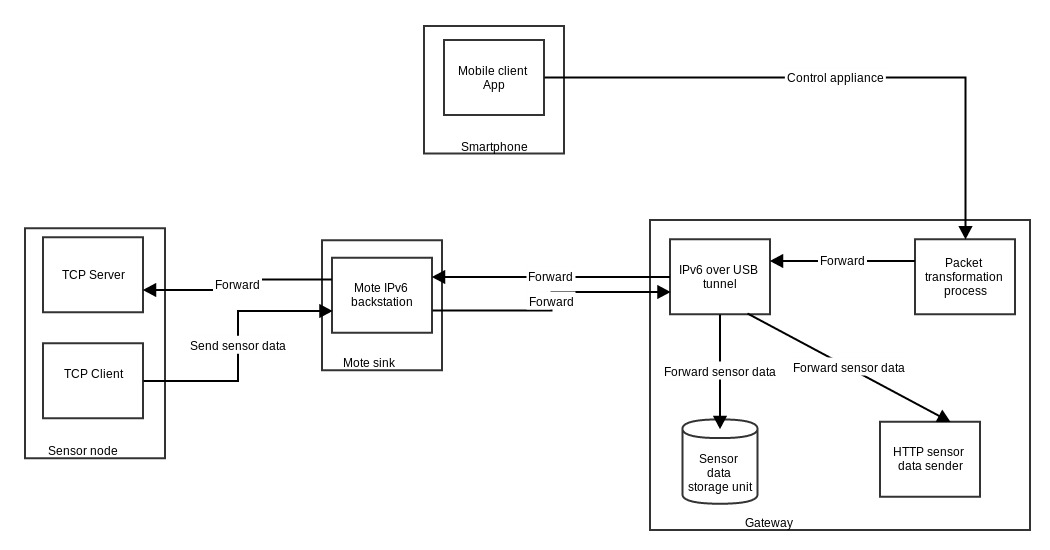
\includegraphics[scale=0.40]{img/general_architecture.jpg}
\caption{General architecture depicting the main components of the system}
\label{fig:gen_architecture}
\end{figure}
\paragraph{}
Now that the general architecture has been defined, the question that should be asked is whether all these components reside in the same layer in the \gls{osi} model and if not, in which layer does each of these components reside in the \gls{osi} model. As an answer to such a question, figure \ref{fig:layered_view} is here to show on what layer does every component act on.

\begin{figure}[htbp]
\centering
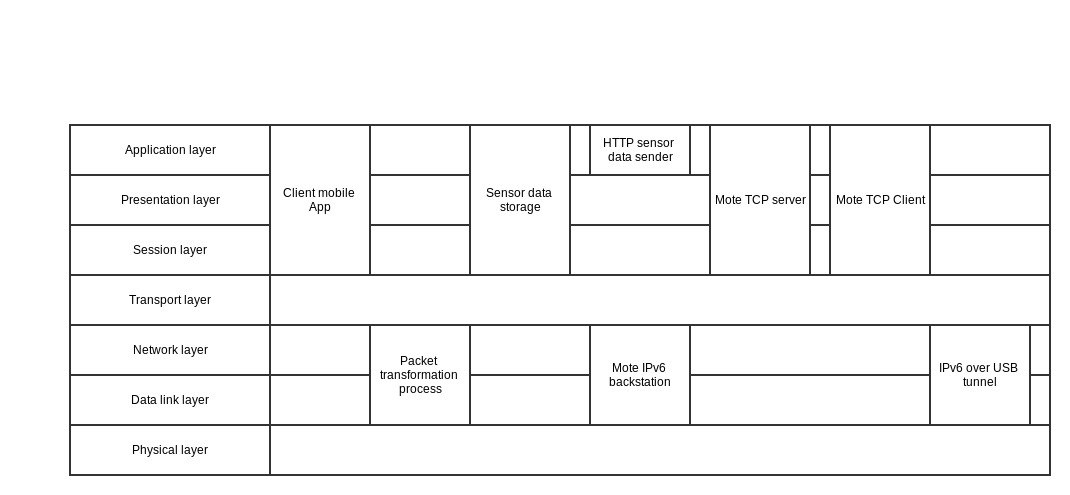
\includegraphics[scale=0.40]{img/layered_view.jpg}
\caption{Layered view showing where every component appears in the \gls{osi} model}
\label{fig:layered_view}
\end{figure}
\paragraph{}
From figure \ref{fig:layered_view}, one can see that there are three components in performing in the data link layer and network layer. The first one is the packet transformation process whose goal is to hide the communication heterogeneity by sniffing incoming packets, transforming them, and forwarding them to the destination to meet the destination's communication technology and standards used. The second component performing in the data link layer and network is the \gls{ipv6} over USB tunnel. This component is in charge of getting raw \gls{ipv6} packets and encapsulate them through USB to reach the destination. The third component is deployed in the mote sink which is the entry and exit point of the \gls{wsn}. This special mote receives \gls{ipv6} packets encapsulated in USB frames that are forwarded to the destination mote using Zigbee.

\paragraph{}
There are four components that perform in the session layer, presentation layer and application layer and are existing in most of the devices needed in the system. The first one is the client mobile App. This component is mostly a TCP client and uses many of the services provided by the layers it is performing on. The second component is the sensor data storage which is a TCP server receiving data from the \gls{wsn} and sending storing it in a \gls{rdbms}. The third and fourth components are the Mote TCP client and Mote TCP server that send sensor data and through the TCP client and receive orders to control the appliance using the TCP server. 
\paragraph{}
The only component acting in the application layer exclusively is the HTTP sensor data sender which provides a gateway to other applications willing to use such data and later on make use of the system. This component receives data and sends to the destination by using HTTP protocol. The middleware application was using HTTP to get sensor data from this system.
\paragraph{}
Now that the general structure of the software system has been established, the hardware structure is to be presented and explained further. figure \ref{fig:network_diagram} is a network diagram that shows the of the hardware components that exist within this system. The \glsreset{wsn}\gls{wsn} appears on the right of the document. Attached to it a mote sink that exist both in the \gls{wsn} and outside it. This mote sink is attached to the gateway server through USB. The gateway has also a Wi-Fi interface card that enables it to communicate with the other parts of the system such as the middleware and the mobile client.

\begin{figure}[htbp]
\centering
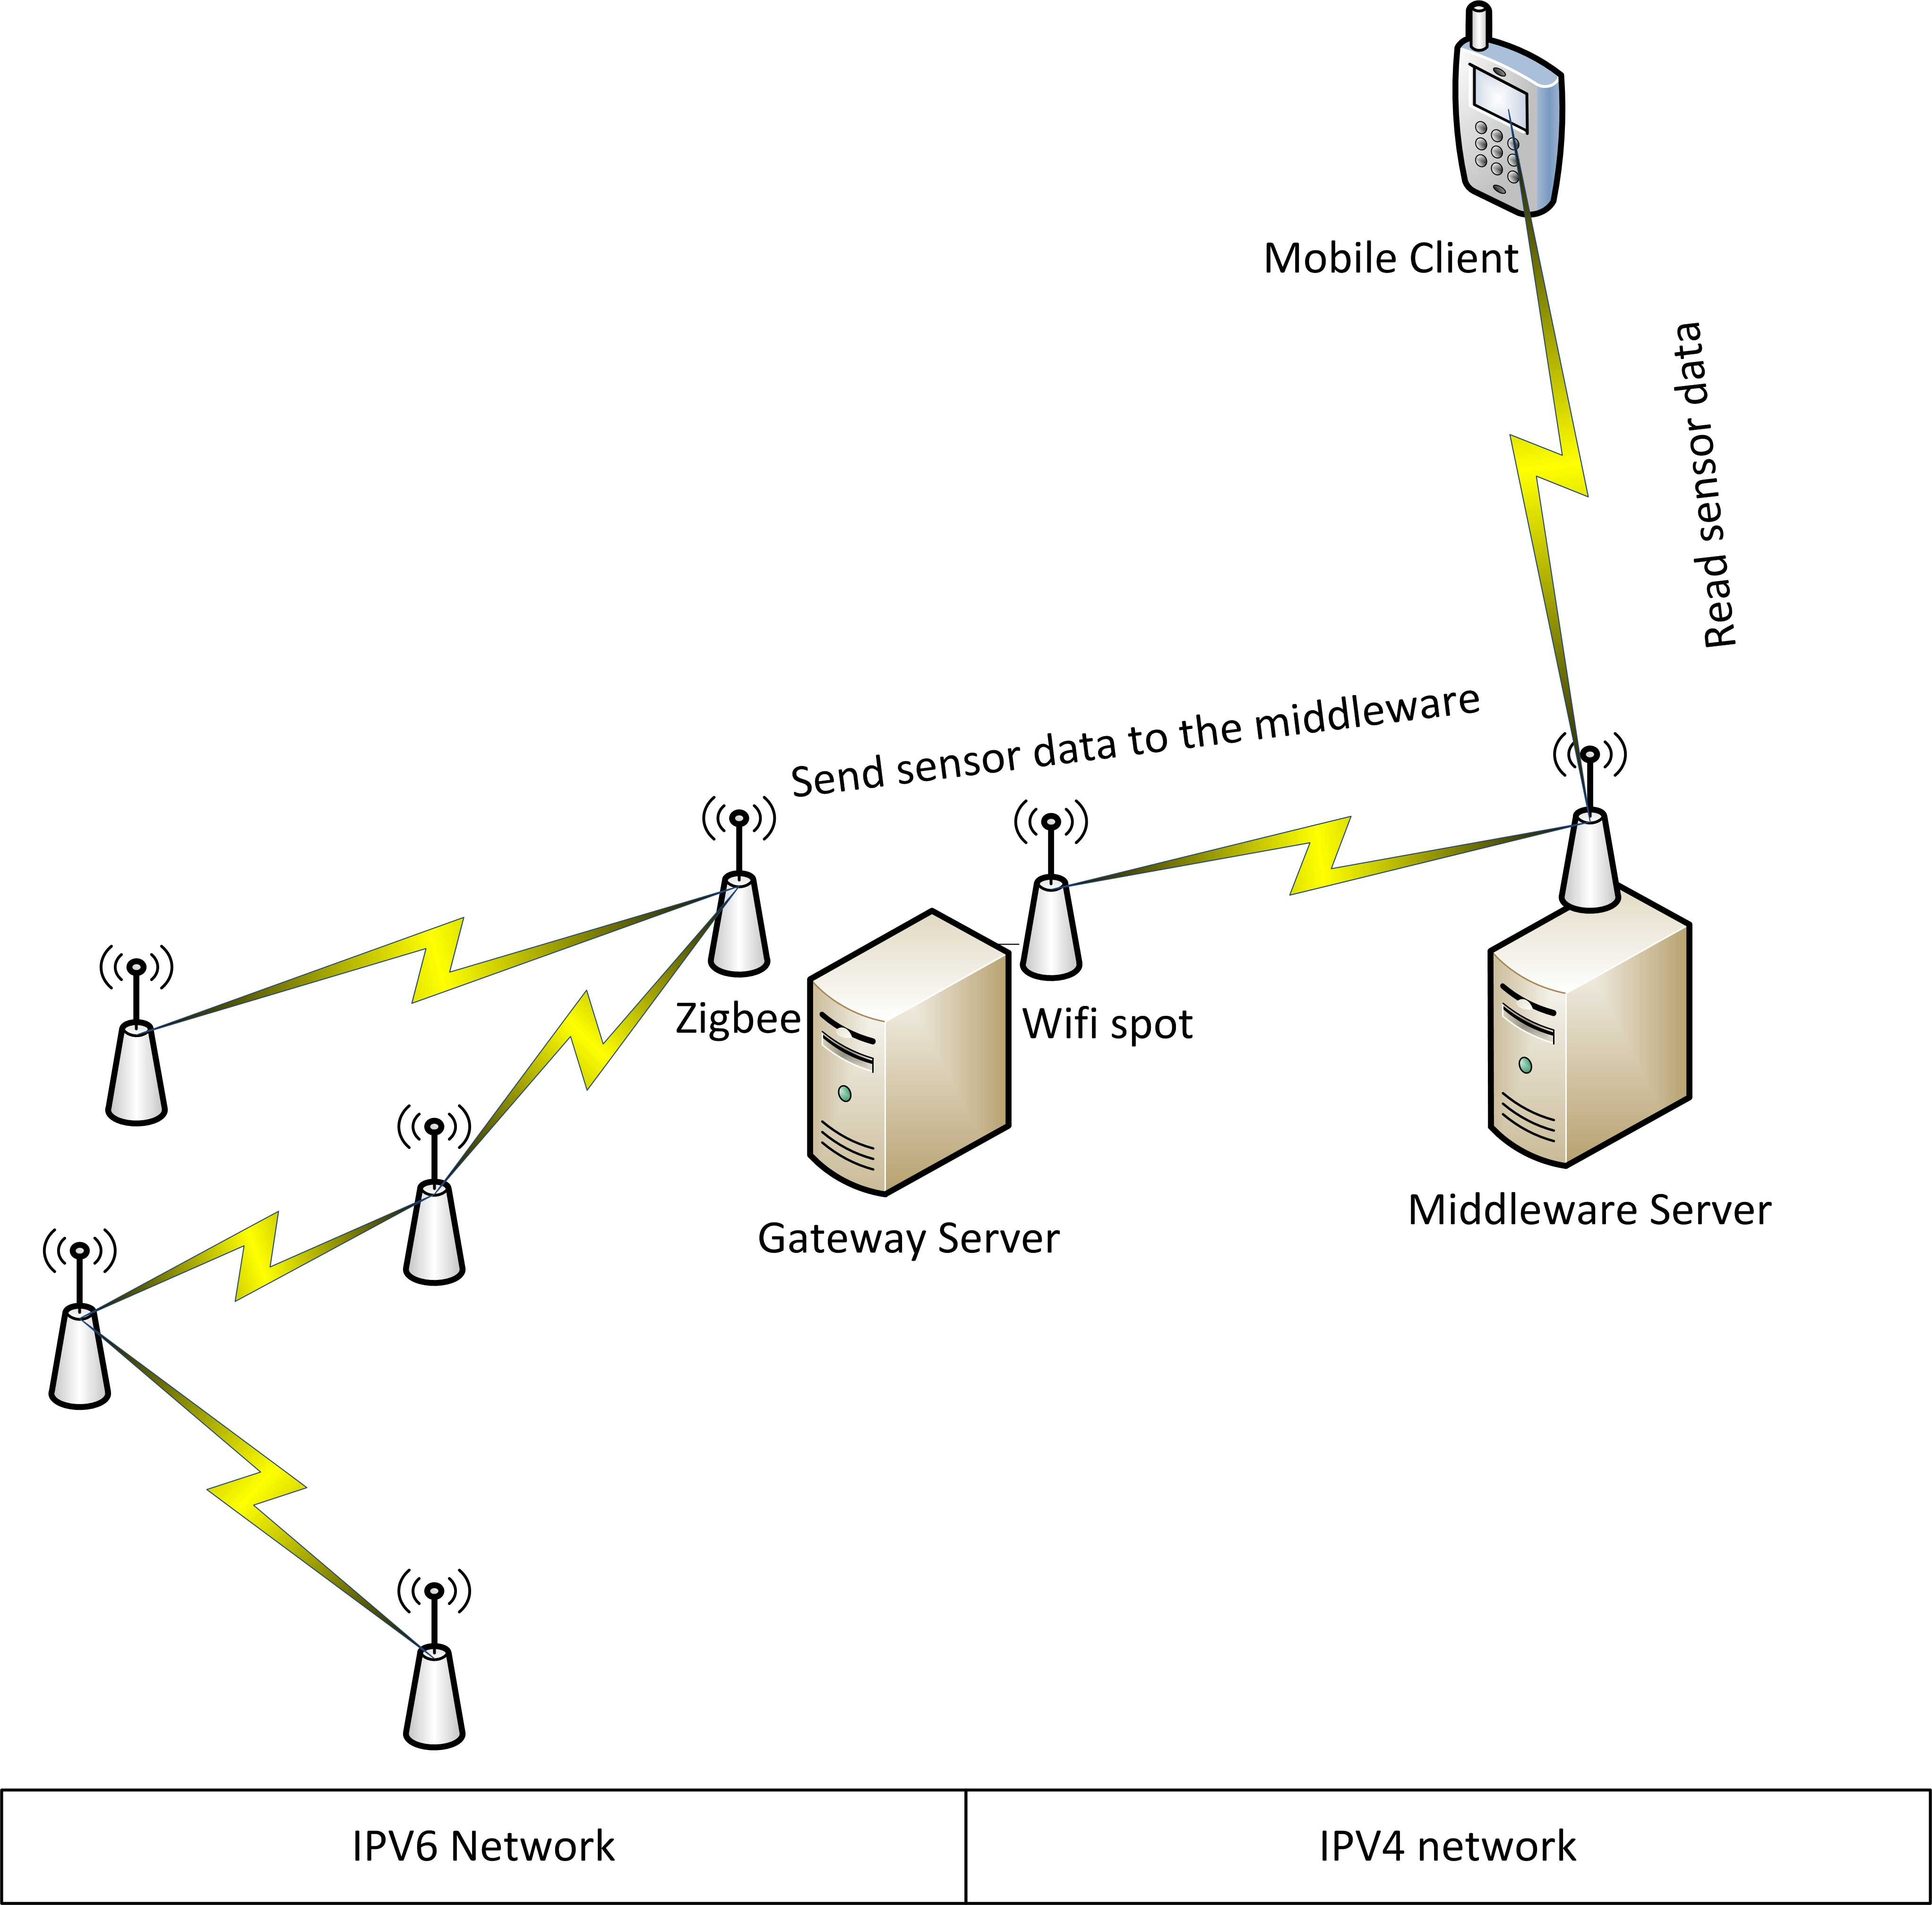
\includegraphics[scale=0.8]{img/network_diagram.jpg}
\caption{Network diagram of the system}
\label{fig:network_diagram}
\end{figure}
\paragraph{}
Now that the network diagram has been established in \ref{fig:network_diagram} where the hardware component appears, the next thing is to show where each software component will be deployed. In other words, what are the software components that exist on which hardware machine. This is the goal of table \ref{table:soft_hard_deployment}. It clearly shows what software components exist in what hardware. From the table \ref{table:soft_hard_deployment}, it is clear that there are hardware machines that have more than one component deployed and this is also the case for small devices such as sensor nodes within the \gls{wsn}.

\begin{table}
    \begin{tabular}{lllll}
    		  \hline
    Software component - Hardware component & Mote & Mote sink & Gateway & Mobile \\ \hline
    Mote sensor data collection TCP client  & X    & X         & ~       & ~      \\ 
    Mote appliance control TCP server       & X    & X         & ~       & ~      \\
    Gateway packet transformation process   & ~    & ~         & X       & ~      \\
    IPv6 over USB tunnel                    & ~    & ~         & X       & ~      \\
    Mote IPv6 backstation                   & ~    & X         & ~       & ~      \\
    Sensor data storage process             & ~    & ~         & X       & ~      \\
    HTTP sensor data sender                 & ~    & ~         & X       & ~      \\
    Mobile client                           & ~    & ~         & ~       & X      \\
    \end{tabular}
    \caption{Software-hardware deployment table}
    \label{table:soft_hard_deployment}
\end{table}
\paragraph{}
In the following sections, each software component will be described in more details showing why such a component is crucial and what are the architectural decisions made to be what it is.

\section{Mote Sensor Data Collection TCP Client}
The mote sensor data collection TCP client is nothing more but a \gls{tcp} client deployed in a mote that is attached to an appliance that reads sensor data periodically from the consumption sensor more known as the \gls{ct}  as showns in figure \ref{fig:current_transformer} that returns after a few transformations of the data the exact amount of power consumer in \gls{wh}. The original amount returned a voltage value in \gls{v} that is then transformed into the electric intensity in \gls{a}. To transform, the voltage into the actual current intensity we make use of the data provided by the \gls{ct} manufacturer. By making use of an experiment whose goals is to measure the slope and the constant of the voltage to intensity function. This function resulted in the following values:

\begin{figure}[htbp]
\centering
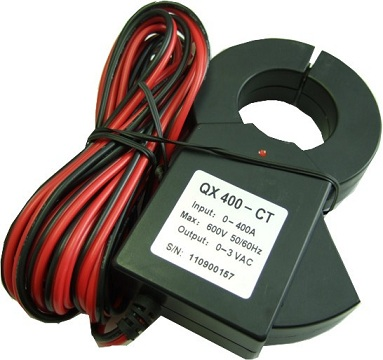
\includegraphics[scale=0.8]{img/ct.jpg}
\caption{Current transformer}
\label{fig:current_transformer}
\end{figure}

\begin{table}
    \begin{tabular}{ll}
    \hline
    slope    & 66.7 \gls{a} \\ \hline
    Constant & 0 \gls{a}    \\ \hline
    \end{tabular}
    \caption{Current Transformer values}
        \label{table:CT_vals}
\end{table}
The transformation function is then: \\
\boldmath{$I = 66.7U_0$} \\
I: Intensity in \glsreset{a}\gls{a} \\
$U_0$: The voltage read from the \gls{ct}

\paragraph{}
Afterwards, as the voltage in Moroccan households is 220 \gls{v} we get the power using the following function:
\\
\boldmath{$ P = U_1 I $} \\
P: Power in \gls{w} \\
I: Intensity in \glsreset{a}\gls{a} \\
$U_1$: Electrical potential difference or Voltage in household in \glsreset{v}\gls{v}
\paragraph{}
P refers to the power, not the actual consumption of the appliance. To get the consumption we use an additional parameter which is the sampling rate. The sampling rate is defined as the number of sensor reading actions per hour. If one reads sensor data every second, then the sampling rate is 3600 samples per second.
\paragraph{}
To find the actual consumption, we need to consecutive sensor readings that we call $P_0$ and $P_1$ and use the following function:
\\
$ C = \cfrac{P_0 + \cfrac{P_1 - P_0}{2}}{S} $ \\
C: Current Consumption in \glsreset{wh}\gls{wh} \\
P: Power sample number 1 in \glsreset{w}\gls{w} \\
P': Power sample number 2 in \glsreset{w}\gls{w} \\
$U_1$: Electrical potential difference or Voltage in households in \glsreset{v}\gls{v} \\
S: Sampling rate \\
The assumption taken is that if the power varies between two consecutive samples, the change was made linear throughout the interval of time between the two.
\paragraph{}
Once the consumption data in hand after this series of transformation, the next thing left to do is to send this data. To send it, the mote make use of the \gls{tcp}  client built on top of \gls{blip} package that implements the TCP/IP protocol stack. The system is made in a way that all the sensor data is sent to the gateway services that will decide to store it in a data store or send it to another system outside of the scope of this project.
\section{ Mote appliance control TCP server}
\paragraph{}
The mote appliance control \glsreset{tcp}\gls{tcp} server is a component that is deployed in the sensor nodes of the \gls{wsn} to get commands from the outside world or at least outside of the \gls{wsn} in order control the appliance attached it. To control an appliance, one has access to two commands which are the ability to turn on and off a device.
\paragraph{}
Figure \ref{fig:appliance_control} depicts the architecture as well as the data flow of the command to turn on/ off an appliance. The TCP server hosted in the mote receives on/off commands from and external TCP client. The command is then extracted from the protocol of communication, and based on that, the PIN is known. the PIN information as well as the functionality is called as it is implemented in the MDA320CA that applies it on the pin and opens or closes the circuit depending on the command specified by the external TCP client.

\begin{figure}[htbp]
\centering
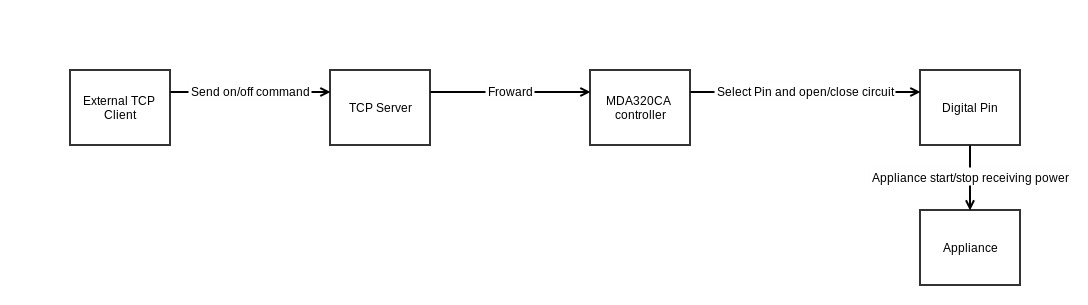
\includegraphics[scale=0.35]{img/appliance_control.jpg}
\caption{TCP Server controling appliance}
\label{fig:appliance_control}
\end{figure}

\paragraph{}
The mote by itself does not have the necessary capabilities needed to control a mote. In order for a mote to have such capabilities, it needs to be equipped with an additional board, a Data Acquisition board also called a extension board that enable the mote to have more capabilities and therefore the ability to control the power flowing into the mote. The extension board used in the course of this project is the Crossbow MDA320CA as depicted in figure \ref{fig:mda320ca}. This board has pins which are electrical inputs and outputs that make it possible to have external analog sensors, digital sensors and also be able to power the appliance. But the powering of the appliances is not as straightforward as it seems especially that sensor nodes are very low-power devices that cannot provide enough energy to appliances such as a television or a fridge.
\paragraph{}
To make a mote control the appliance, the mote will control the power going in a very small circuit and this circuit is responsible for letting the power flow through the appliance from another source of energy which is naturally far more important than the one provided in the mote. In summary, the mote has a the extension board of type MDA320CA that has a small electric circuit attached to one of its digital pins that then controls the flow of electricity going to the appliance. By turning off a pin, the electricity stops flowing through the circuit and becomes open which stops the electricity to go to the appliance. 

\begin{figure}[htbp]
\centering
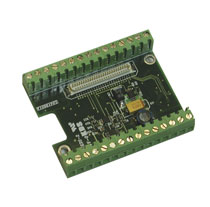
\includegraphics[scale=0.8]{img/mda320.jpg}
\caption{Crossbow MDA320CA Data acquisition board}
\label{fig:mda320ca}
\end{figure}

\section{Mote IPv6 Backstation}
\paragraph{} 
This component that exist in one special mote in the \glsreset{wsn}\gls{wsn}. This mote is able to communicate with the rest of the \gls{wsn} using Zigbee and also with the external world using \gls{usb}. This make this mote a sink and a router because it has two interface cards. The software component deployed in this sink is a packet forwarder. This means that once it receives an \gls{ipv6} packet that is not in the \gls{wsn}, it is forwarded through \gls{usb}.
\paragraph{}
The mote's sole goal is forwarding packets in and outside of the \gls{wsn} while other sensor node do not need to worry about how the packet will arrive to its destination. This mote is part of the components aiming to solve the heterogeneity problem stated in the problem statement. By making the sensor nodes talk to any device as if it is part of the \gls{wsn}, they do not really have to worry about how it will arrive or even how did the packet get to them in the first place.

\section{IPv6 over USB Tunnel}
\paragraph{}
The gateway server machine is equipped with two interface cards: the Wi-Fi network interface card and the Zigbee network interface card. The Zigbee network interface card is the one on focus in this section. To have a device communicating using Zigbee, one sensor node within the \gls{wsn} was used for this purpose and the software component implemented in this sensor node is the one described in section 4.6. That said, the packet is received through \gls{usb} but not read and recognized as a packet by the TCP/IP protocol stack. To do so, a tunnel had to be created for the purpose of extracting packets from the \gls{usb} port. Another goal is to forward \gls{ipv6} packets through that same \gls{usb} and this can only be done by the use of an \gls{ipv6} over \gls{usb} tunnel. 

\section{Gateway Packet Transformation Process}
The gateway packet transformation process is one of the main components that hide the heterogeneity from the rest of the system and the outside world. This component mainly deals with packet transformation which means that it extracts the data from the packet and create a completely new one that holds the data and forward it. This component is composed of three subcomponents:
\begin{itemize}
\item Packet sniffer
\item Packet transformer
\item Address translator
\end{itemize}
\paragraph{}
Figure \ref{fig:gateway_transformation} depicts the architecture of this component by showing the the different subcomponents that reside in this component and their interaction. It also shows the data flow within this component and what are the inputs and outputs of the system.

\begin{figure}[htbp]
\centering
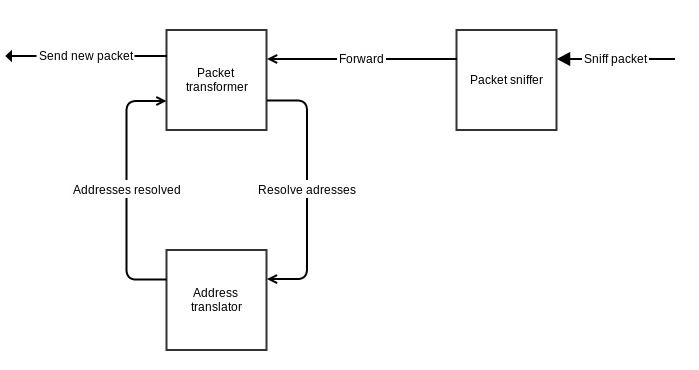
\includegraphics[scale=0.6]{img/packet_transformation.jpg}
\caption{Gateway packet transformation subsystem data flow}
\label{fig:gateway_transformation}
\end{figure}
\paragraph{}
The subsections 4.8.1 - 4.8.3 will go more into details in explaining the three subcomponents of the system.

\subsection{Packet Sniffer}
\paragraph{}
The packet sniffer subcomponent is the one responsible for sniffing and forwarding the packets to the component. It does not forward all the packets that are not going to the gateway machine. In other words, all the packets that are not meant to be received by the gateway server are sniffed and forwarded to the packet transformer that will continue the work.
\subsection{Packet Transformer}
\paragraph{}
Once the packet is received, the first thing this subcomponent does is check from where did it come, was it from the \gls{wsn} or the outside world. If it came from the outside world, the packet will only be examined if it is meant to go the \gls{wsn}. But an important and crucial problem presents itself:
\paragraph{Problem}
\underline{The outside world mostly uses \gls{ipv4} whereas the \gls{wsn} uses exclusively \gls{ipv6}} \\
Two networks using different network layer technology cannot communicate even though \gls{ipv6} is nothing more but a new version of the very known \gls{ipv4} and this is because \gls{ipv6} has no backward compatibility with \gls{ipv4}.
\paragraph{Solution}
To solve such a problem, we decide to provide all the nodes in the this system with both an \gls{ipv4} and \gls{ipv6} address. Some of the nodes have either \gls{ipv4} or \gls{ipv6} addresses, but for the technology missing we assign the missing one virtually. For example, a sensor node in the \gls{wsn} with a real \gls{ipv6} address equal to FEC0::1 will be assigned a virtual \gls{ipv4} address equal to 192.168.0.1 but he will not be aware of it. Only the Gateway packet transformation component will be aware of it and this is the mechanism used to transform the packets and hide the heterogeneity from the rest of the components of the system.
\paragraph{}
Now that a packet is received, it checks whether this component came from the \gls{wsn} or the outside world, depending on that, it extracts the data from the packet which can be a \gls{tcp} or \gls{udp} datagram. The source and destination addresses are extracted from the packet and translated to the other network technology. Afterwards, a new packet referring to the destination technology used is created by having as a source and destination addresses the translated addresses and as payload the the \gls{tcp} \gls{udp} datagram coming from the original packet. Finally, the packet is forwarded to the network.
\subsection{Address Translator}
The address translator is a very specialized subcomponent whose sole goal is to translate addresses between \gls{ipv4} and \gls{ipv6}. That is said, this component receives the address to translate and returns the translated one. Its concern is that the translation algorithm yields a bijective function which means that for any \gls{ipv4} address there is one and only one \gls{ipv6} address resulting from that source and vice versa. This statement compresses a set of statements which are the following:

\begin{itemize}
\item Any address belonging to one technology can be translated to the other technology. This is known as surjectivity.
\item Any address cannot be translated into more than one address from the other technology. This is known as injectivity.
\end{itemize}
\paragraph{}
The gateway packet transformation process is an important component responsible for dealing with the heterogeneity problem. It hides most of the heterogeneity in the system and make communication go independently of the data link layer or network layer technologies used.

\section{Sensor Data Storage Process}
\paragraph{}
The sensor data storage process is a component small component within the system whose sole purpose is to store such data. It seen by the \gls{wsn} as a TCP server, where sensor nodes get connected to it as soon as they are turned ON. The sensor node starts sending packet periodically (depending on the sampling rate specified) and whenever the sensor data is received, it is stored into a \gls{rdbms} where the schema is created as shown in figure \ref{fig:erd}.

\begin{figure}[htbp]
\centering
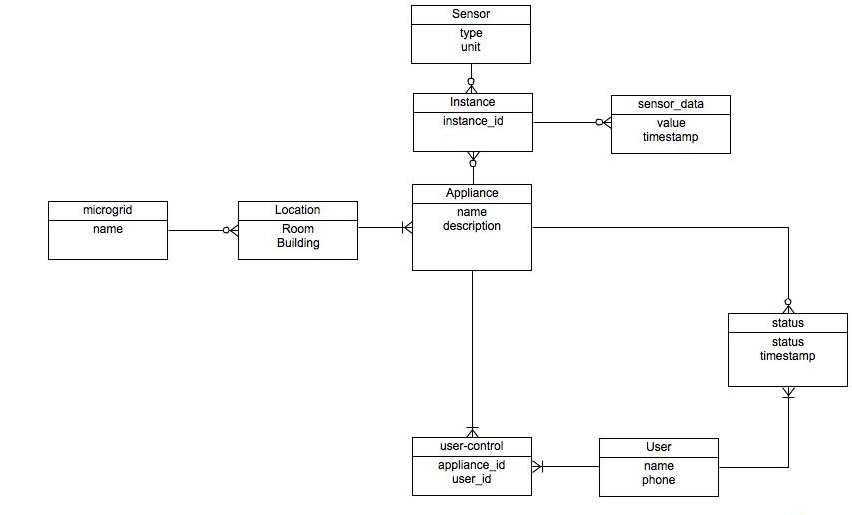
\includegraphics[scale=0.5]{img/smart_grid_db.jpg}
\caption{Entity relationship diagram}
\label{fig:erd}
\end{figure}

\section{HTTP Sensor Data Sender} 
The HTTP sensor data sender is TCP server to which sensor nodes get connected to and start sending their data periodically. Once the data is received they are able to send data to the outside world periodically depending on the needs of the clients outside the system. This system counts on the deployment of an HTTP server at the level of outside the system client and send an HTTP request containing the sensor data received from the \gls{wsn}. 
\paragraph{}
The sensor nodes are able to send this data by themselves directly to the outside as this is part of the two-way communication but for convenience, it was decided that the \gls{wsn} sends its data to the gateway and it is up to the gateway to send such data or store it in the \gls{rdbms}.
\section{Mobile Client}
The mobile client is a component of the system but can be seen as an outside world client as it is here to receive sensor data and also send ON/OFF commands to the system.

\chapter{Deployment}
\paragraph{}
In this chapter, the test-bed will be discussed from the implementation point of view. That is said, each component within the system will be given as much details as possible in order for the reader to open the code and understand what is going. Chapter 4 discussed the components from the architectural aspect but no implementation and technology decisions were discussed and the goal of this chapter is to explain these details.
\section{Technology Enablers}
The system's implementation was built using a set of software and hardware technologies and standards that were used throughout the course of this project to make the test-bed achieve its objectives.
%\glsreset{wsn}
\subsection{Technologies used in \gls{wsn}}

\begin{figure}[htbp]
\centering
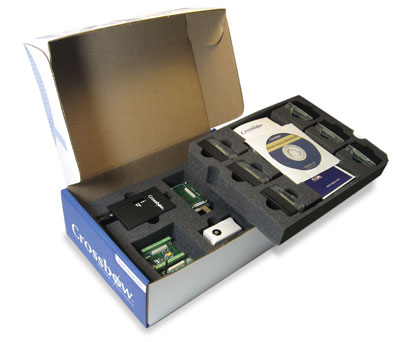
\includegraphics[scale=0.6]{img/crossbow.jpg}
\caption{Crossbow Professional Kit}
\label{fig:crossbow}
\end{figure}

The \gls{wsn} was built using Crossbow professional kit as shown in figure \ref{fig:crossbow} which counts 7 Micaz sensor nodes of type MPR2600 as shows in figure \ref{fig:micaz}.
\begin{figure}[htbp]
\centering
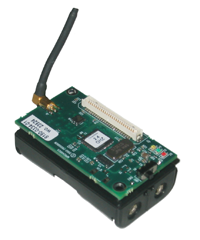
\includegraphics[scale=0.8]{img/micaz.png}
\caption{Crossbow MPR2600 Micaz Mote}
\label{fig:micaz}
\end{figure}

In addition, each mote is supplied with a sensor board of type Crossbow MTS400CA which contains temperature, humidity, barometric pressure, ambient light and infrared light sensors that are used to send different types of sensor data to the gateway. This board is shown in figure \ref{fig:mts400}.

\begin{figure}[htbp]
\centering
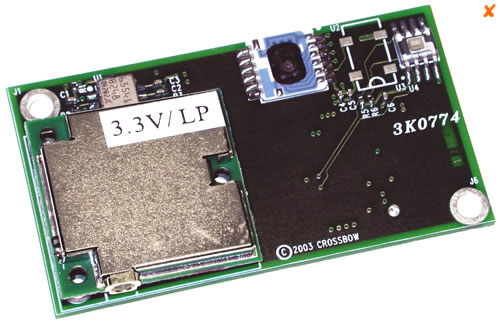
\includegraphics[scale=0.5]{img/mts400ca.jpg}
\caption{Crossbow MTS400CA Sensor Board}
\label{fig:mts400}
\end{figure}
\paragraph{}
The WSN is run using \gls{tinyos} which is one of the most used opensource \gls{os} in \glspl{wsn}. Programs are implemented using \gls{nesc} which is the sole programming language used in the \gls{tinyos} environment. This programming language is event-oriented and its syntax is very influenced by C. In addition, C libraries can be used in \gls{nesc} programs.

\subsection{Technologies used in the Gateway}
\paragraph{}
The gateway's hardware machine is Dell Optiplex 9010 running a Linux environment more specifically the Ubuntu 13.04 distribution. The gateway has a set of technologies used to provide numerous services the system counts on. The programming languages used in the components hosted in this machine are C and \gls{j2se}. Netfilter is also used to control incoming and outgoing packets. Concerning the storage of sensor data MySQl is the \gls{rdbms} used.

\subsection{Technologies used in the Mobile Client}
\paragraph{}
The mobile used is an Android smart phone with Android 2.3. The application developed is using \gls{j2se}, PHP for database connectivity.

\section{Mote TCP Client And TCP Server}
\paragraph{}
Section 4.4 and 4.5 were dedicated to explain the TCP Client and TCP server separately. In this section, one section will explain both of them because from the implementation point of view,  both of them are implemented in the \gls{tinyos} program.
\paragraph{}
A typical \gls{tinyos} program has two parts: the components definition part and the module part. In the components definition part, the main components that will be used. These components refer to already implemented modules whose functionalities will be used in the in-development module. In the module part, we provide define the interfaces we will be using and the interfaces we will be providing if any \cite{ref14}. Back to definition part, after defining components we will be using, we then link the interfaces needed in the module to the components providing that interface. This is known as wiring.
\paragraph{}
The components needed in this program are the following:
\begin{itemize}
\item MainC: provides the essential functionalities such as the initialization and closing of the program.
\item LedsC: provides access to the leds existing in the mote
\item Taos2550C: is a light sensor component that enable to read data
\item TimerMillic: A Timer that will be used for sampling
\item TCPSocket as client: Is the TCP client
\item TCPSocket as Server: Is the TCP server
\end{itemize}
In the modules part we define the components that will be used which are the following:
\begin{itemize}
\item Boot: This is the interface that provides main functions of booting and closing
\item TCP as server: The main interface for TCP
\item TCP as client: The main interface for TCP
\item Leds: The interface to access the leds
\item timer as sensingTimer: The interface to program and use the timer
\item Read as Sensor: The interface to talk with the sensor
\end{itemize}
Some of the interface do not have all the functions provided and the not implemented function are implemented in the module. The following part will talk about each function that is to be implemented
\paragraph{After boot of the mote}
The first thing done after the mote is booted is to initialize the TCP client and server. The Client is given a random port by using the rand function. The TCP server is binded to port 7. The client is set to connect to the Data store in the gateway by providing the \gls{ipv6} address of the gateway and port number of the server. Afterwards, the timer is set to be triggered every 10 seconds which means that the sampling rate will be 360 sensor readings per hour. 
\paragraph{TCP Server data received}
Once the data is received from a client, it assumes that there are two data items separated by a space. The first item refers to the led number(1,2,3) and the second refers to the command 0 meaning turn Off and 1 means turn On. The string is tokenized and the data items are extracted and the command is executed accordingly.
\paragraph{Timer fired}
Once the timer is fired, this means it is time to read sensor data from the sensor. The command to read from the sensor is called which goes and reads data and once the data is read the event "read done" is triggered.
\paragraph{Read done}
Once the data is read and ready, the next thing is to transform it and then send it. Concerning the transformation, a series of equations are applied as seen in section 4.4 which build the data value from the original value gotten and it is ready to be sent. A message is created containing two values: the mote NODE\_ID which is the identifier of the mote predefined in the installation of the program in the mote and the sensor data value. These two values are separated by a space, encapsulated within a \gls{tcp} datagram and sent.
\paragraph{}
During the installation of the software the \glsreset{blip}\gls{blip} package should specified as it is a dependency of the software system. \gls{blip} provides the TCP/IP protocol stack that implements \gls{6lowpan} standard by \gls{ietf}. In  the installation the NODE\_ID is specified. If NODE\_ID is 1, this will make the mote have an \gls{ipv6} of FEC0::1, as the NODE\_ID is appended to the predefined prefix of \gls{wsn} during the installation.
\section{Mote IPv6 Backstation}
\paragraph{}
This component is provided as part of the \gls{blip} software package. It is \gls{tinyos} program whose goal is to forward packet back and forth between the \gls{wsn} and the outside. This mote is connected to the \gls{wsn} using Zigbee and to the outside world using \gls{usb}. This special mote has its \gls{ipv6} being FEC0::64. It receives \gls{ipv6} packets encapsulated in \gls{usb} frames, extracts them and encapsulates them in a Zigbee frame and vice versa.
\paragraph{}
During the installation of this \gls{tinyos} program into the mote sink, one should make sure that it is being installed in the mote sink as \gls{usb} is a necessity. The \gls{ipv6} address does not need to be provided as it is already predefined in the program.

\section{IPv6 over USB Tunnel}
\paragraph{}
This is a program that is installed in the gateway server machine. As the mote sink is connected to the gateway using \gls{usb}, the gateway will recognize it as a network interface card using \gls{ipv6} as a network technology. That is said, this component is part of the \gls{blip} software package and creates the network interface card module and starts extracting incoming \gls{ipv6} packets from the \gls{usb} frames and encapsulates outgoing \gls{ipv6} into \gls{usb} frames.
\paragraph{}
The installation and initialization of this component will be given more details in appendix A.
\section{Gateway Packet Transformation Process}
\paragraph{}
This component is in charge of hiding the heterogeneity of the system from the rest of the the components of the system and also the outside world. It does that by intercepting all the packet moving and transforms them according to the standards used by the recipient.
\paragraph{}
The program works with Netfilter in parallel. This means that Netfilter should drop all incoming and this program will take care of dealing with incoming packets separately. 
\paragraph{}
To make use of this process, there is an initial configuration that should be done to all the components of the system in order for the system to work. The gateway has two network interface cards: the Wi-Fi interface and the Zigbee interface provided through the tunnel. The first one is using \gls{ipv4} and the second is using \gls{ipv6}.
\paragraph{}
The program has three subcomponents as seen in section 4.8. The three components are the following:
\begin{itemize}
\item Packet sniffer
\item Packet transformer
\item Address translator
\end{itemize}
The following subsections will discuss each of these subcomponent separately from the implementation point of view.

\subsection{Packet sniffer}
\paragraph{}
The packet sniffer is the one in charge of sniffing packet from both network interface card, as Raw Frames. The code snippet shows the functions called to sniff the packets. We make use of the raw socket library that enables us to sniff data link layer frames before being dropped by Netfilter.
The main reason of dropping the packets by Netfilter is that the packets will not addressed to the computer and therefore the computer make send ICMP messages to the sender saying that the route is not the best and therefore the sender will never send packets again which is something we need to avoid to have.

\begin{lstlisting}
sockfd = socket( PF_PACKET, SOCK_PACKET , htons(ETH_P_ALL));
if (sockfd < 0)
	exit(1);
	
while(1)
{
	data_size = recvfrom(sockfd,buf,10000,0
		,(struct sockaddr *)&cliaddr,&clilen);
}

\end{lstlisting}
\paragraph{}
The first line of code is the initialization of the raw socket, we define the type, scope and name space of the packets to be sniffed. This will return a file descriptor that will allow us to call the socket. Afterwards, we start reading packets in an infinite loop.

\paragraph{}
After sniffing a packet, we must check if it is an \gls{ipv4} or \gls{ipv6} packet. The problem is that when reading from the Wi-Fi interface card, we get the whole frame where the network packet is encapsulated, but the Zigbee Tunnel only gives the raw \gls{ipv6} packet. Once a packet is read by the frame, from which interface card came is a problem and therefore a partial solution is found. We cast the packet to Wi-Fi frame and whenever we check for the network protocol, we get two solutions, 0 referring to \gls{ipv6} and 8 referring to \gls{ipv4}.
If we get zero, the whole data should be casted to the \gls{ipv6} data structure whereas if it is 8, we should move the pointer forward to drop the Wi-Fi header and cast the following part to the \gls{ipv4} data structure.
\paragraph{}
In each of those conditions we only select the TCP datagrams and this is why we check if the next header in the IP structure is equal to 6. After that we move the pointer to drop the IP header and only keep the TCP datagram that will have to be sent in a the newly transformed packet. Depending on the network technology of the sniffed packet, we should build a new packet with the technology that is recognized by the recipient.

\begin{lstlisting}
if(header->h_proto == 0) 
{
	if(ip6_hdr->ip6_nxt == 6)
	{
			buf += IP6_HDRLEN;
			... 			
			sendIPV4Packet(..)
	}
}
else if(header->h_proto == 8)
{
	if(ip_hdr->protocol == 6)
	{
		buf += (sizeof(struct ethhdr)+ IP4_HDRLEN);		
		...
		sendIPV6Packet(...)
	}
}
\end{lstlisting}

\subsection{Packet transformer}
\paragraph{}
The packet tranformer subcomponent is in charge of building two types of packets: \gls{ipv4} and \gls{ipv6} packets. As stated in section 4.8, all devices in this system have an \gls{ipv4} and \gls{ipv6} address where one of them is not recognized only at the gateway. As the \gls{wsn} excelusively supports \gls{ipv6} and they cannot be addressed without using their \gls{ipv6} address and any other device not using \gls{ipv6} may communicate with them by using their virtual \gls{ipv4} address at once the packets reach the gateway, it transform so that the data carried will be delivered and the packet will have instead of \gls{ipv4} source and destination addresses, \gls{ipv6} addresses that will be translated using the Address translator subcomponent.
\paragraph{}
This subcomponent is based on two important functions:
\begin{itemize}
\item sendIPv6Packet(..)
\item sendIPv4Packet(..)
\end{itemize}
\paragraph{}
The idea is the same for except that each technology has its own details such as filling different fields and computing the checksum. Another difference is when creating the \gls{ipv4} one should also create the Wi-Fi frame otherwise it won't be able to be sent through the corresponding network interface card whereas when building \gls{ipv6} packet one should just send the packet and the tunnel will take care of encapsulating it into a \gls{usb} frame.
The function receives the data to be sent which is in all cases a \gls{tcp} datagram along with the size of the datagram, the source and destination addresses that are already translated. Afterwards, the transformator creates the packet appends the datagram, fills the source and destination address and create a socket attached to the corresponding interface card and send the packet.
\begin{lstlisting}
int sendIPV6Packet(char* buffer,int size,char *src ,char *dest)
{
	//CREATE PACKET WITH ALL ITS DETAILS
	...
	memcpy (frame + IP6_HDRLEN, buffer, size);
	sd = socket (PF_PACKET, SOCK_RAW, htons (ETH_P_ALL))) < 0);
	sendto (sd, rame, length...);
}
\end{lstlisting}

\subsection{Address translator}
\paragraph{}
The address translator is the subcomponent that assigns \gls{ipv4} and \gls{ipv6} to all devices in this system. For instance, sensor nodes in the \gls{wsn} have \gls{ipv6} addresses but this subcomponent assigns to them \gls{ipv4} addresses.
\paragraph{}
To do so, the translation algorithm is purely bijective. That is said, any \gls{ipv4} is translated to one and only one \gls{ipv6} and vice versa. For a mobile client with \gls{ipv4} address of 10.50.1.50 to talk with a mote whose \gls{ipv6} address is FEC0::1, the mobile client should be aware of its translated to \gls{ipv4} address which is 192.168.0.1. Once the packet is received and knowing it is not addressed to it. The source and destination \gls{ipv4} addresses are translated to \gls{ipv6} making the source address equal to 0A32::0132 and the destination FEC0::1. The \gls{ipv6} packet is created and reaches the destination which is the sensor node. Once the response is going back the scenario is the same.
\paragraph{}
The translation algorithm has been tested extensively to make sure it is bijective and that any address can be translated to one and no more and than one address. When configuring the system, one should make sure that there is no two devices that have the same address real or virtual. Any \gls{ipv6} and \gls{ipv4} should be unique throughout the whole system. The \gls{wsn} should be granted an interval of \gls{ipv4} address so that no one will be able to have them besides the \gls{wsn} that uses them virtually.


\chapter{Findings}
\paragraph{}
The system was built to provide monitor and control home appliances and also provide an infrastructure for future platforms to be integrated in this system. Such infrastructures can be the integration of the \glsreset{dr}\gls{dr}. To build overlying system's, one should make sure that the system has a certain level of performance that one can count on to build overlying services. The purpose of this chapter is to measure the performance of the system. It is done by first doing and experiment which will help us gather data and then based on this data, an interpretation of this data will be done to see whether the system is shows an acceptable level of performance.
\section{Experiment}
\paragraph{}
To measure the performance of the system, an experiment was conducted where the goal is to quantify the performance of the system. \gls{6lowpan} was built in order for the mote receiving the packet to forward it is not directed to it before dealing with the one directed to it. This means that there is more priority given to routed packet that the processed ones. As a result, this clearly pushes us to think that the delay of the system will not be much affected as the traffic in the network grows.
\paragraph{Experiment 1:}
We will first have one mote in the \gls{wsn} that will be interacting with the outside world. We will start sending ping command periodically (once every 1 second) and record the delay and the jitter. Once every two minutes, we will add another mote to the system and continue pinging the same mote. We keep adding motes every 2 minutes until we fill the \gls{wsn} with 6 motes which is the maximum number of motes available in the system. This will enable us to collect data about the mote delay and jitter as we add more traffic to the system.
\paragraph{Experiment 2: }
The second experience is meant to measure the time it takes to transform the packet. In other words, measure the average delay and jitter that is added when having the Gateway Transformation Process as part of the system. The timer starts before the sniffing of the packet and ends right after the packet is transformed and sent.
We believe that there will be an additional delay to the communication but we are hoping that it will not affect much the whole delay of the communication between different components of the system. 
\section{Data Gathering}
\paragraph{}
After both experiments were conducted, we collected a significant amount of data that was used to measure the performance and an interpretation was done in section 6.3 to have an idea about the performance of the system.
\subsection{Experiment 1}
\paragraph{}
In the first experiment, the same mote was pinged once every second and we added new motes to the system every two minutes. The experiment as a whole took 12 minutes and 720 pings we done. Table \ref{table:exp1} shows the result of the experiment.

\begin{table}[htbp]
    \begin{tabular}{lll}
    \hline
    number of motes & Delay (ms) & Jitter (ms) \\\hline
    1               & 87.5         & 1.2         \\ 
    2               & 88.1         & 2.0         \\
    3               & 88.3        & 2.7         \\
    4               & 88.8         & 3.1         \\
    5               & 90.0         & 3.3         \\
    6               & 89.5         & 3.5         \\
    \end{tabular}
    \caption{Experiment 1 delay and jitter}
    \label{table:exp1}
\end{table}
\paragraph{}
For each row in the table, the average delay is computed using the pings that were performed in the 2 minutes interval which means 120 pings per row. The jitter is also computed in a similar as the average variation from the mean delay in that 2 minutes interval. The result is displayed in the table \ref{table:exp1}. 

\subsection{Experiment 2}
\paragraph{}
The second experiment's goal is to measure the additional delay coming from the Gateway Packet transformation process whose goal to handle and hide the heterogeneity of the system. The result gathered reflects the average delay and jitter computed over elapsed time from the sniffing of the packet to the transformation and sending to the recipient. Table \ref{table:exp2} shows the result that was collected from this experiment as it was done on 200 packets that were sniffed and transformed by the system.

\begin{table}[htbp]
    \begin{tabular}{ll}
    \hline
    Delay (ms) & Jitter (ms) \\ \hline
    0.1        & 0.0         \\ 
    \end{tabular}
    \caption{Experiment 2 delay and jitter}
        \label{table:exp2}
\end{table}
\paragraph{}
The transformation process's elapsed time is counted in nanoseconds and from \ref{table:exp2}, we can see that the average delay is on average 0.1 milliseconds whereas the jitter is 0 milliseconds meaning that the process's time varies between a few nanoseconds to at most 150 nanoseconds. Depending on the machine's load.
\section{Interpretation of Results}
\subsection{Experiment 1}
\paragraph{}
The data collected in section 6.2 shows that the performance of the system is very good. Even though the delay in the \gls{wsn} is high, 
 nothing can be done about that as even though the traffic in the \gls{wsn} is low, the delay is still high and this has to do with the computational time taken by the TCP/IP protocol protocol stack provided implemented by \glsreset{blip}\gls{blip} using \glsreset{6lowpan}\gls{6lowpan}. To reduce the delay, one should probably rethink the design of the \gls{blip} or find a way to omit it, but that is not a good idea since we want the \gls{wsn} to be part of \gls{iot}. 
 \paragraph{}
 The good news in experiment 1 is that the privatization of packets brings benefit to the network. Even though the traffic grows exponentially, the delay does not grow much and the even if the jitter follows to some extent the traffic's trend but still the average delay shows good result. 
 \subsection{Experiment 2}
 \paragraph{}
 The Packet transformation process is a component that shows excellent results. Before conducting experiment 2, we were persuaded that there will be additional delay originating from this process and it could be responsible for the high delay seen in experiment 2 but the results shows otherwise and that the component is not to be put responsible for such important delay seen in experiment 1.
\chapter{Conclusion}
\paragraph{}
This project enabled us to establish an infrastructure as part of the \glsreset{iot}\gls{iot} and move towards having the smart home system's integrated within the smart. At this stage and counting solely on this work, one cannot clearly see the integration of smart home systems within the \gls{iot}, but this is an infrastructure that provides two main services which are the establishment of the two-way communication between the smart home devices and the outside world which may be the utility for instance. This two-way communication enables the \glsreset{wsn}\gls{wsn} to monitor home appliances and send sensor data to a repository which monitors the home's consumption and this device can be used for simulating a real world \gls{ami}. The other part of the communication is the ability of clients to control appliances status by turning them On and Off.
\paragraph{}
The second contribution of this work the smart management of the heterogeneity. The communication from the mote to the mobile client is built on a set of technologies and the journey of a simple \gls{tcp} datagram move through many different data link layer standards and different network technologies. Starting from the mote sending sensor data, The TCP data is encapsulated into an \gls{ipv6} packet that is encapsulated into a Zigbee frame. Afterward, the packet is extracted from the Zigbee frame and encapsulated into a \gls{usb} frame. Once it arrives to the gateway, the \gls{tcp} datagram is extracted from the \gls{ipv6} which is extracted from the \gls{usb} frame and encapsulated in an \gls{ipv4} packet that encapsulated into a Wi-Fi frame and sent until it reaches the mobile. That is said, it clear that the system is heterogeneous and making this heterogeneity transparent was a contribution of this work.
\paragraph{}
The \glsreset{wsn}\gls{wsn} was built making use of the very recent \glsreset{6lowpan}\gls{6lowpan} whose goal is to provide the TCP/IP protocol stack to the smallest devices. The \gls{wsn} is autonomous in the sense that it can work independently and indefinitely by monitoring the home appliances. 
\paragraph{}
All in all, this project as a big picture is a testbed providing the main components of a smart home management with an intelligent \gls{wsn}, a robust and powerful middleware application that is able to use the sensory data and use it to control the home's appliances and a mobile application able to provide the users remote monitoring of their smart homes and control. This was possible by making the system as part of the \glsreset{iot}\gls{iot}.
\chapter{Future Work}
\paragraph{}
This thesis project's was to establish the infrastructure for integrating smart home within \glsreset{sg}\gls{sg} and make it part of the \glsreset{iot}\gls{iot}. This project enabled the deployment of the two-way communication as an infrastructure that can be used to build the \glsreset{dr}\gls{dr}. \gls{dr} is one of the most important topics in smart grids. It enables the utility and households to communicate with a set of services that any of them may request from the other. The current state of the art does not incorporate this communication as part of the smart home systems \cite{ref15}. But as there is a need for this communication, \gls{dr} will have to be implemented as part of the smart home package.
\paragraph{}
Demand reponse integration is a future work for this study. \gls{dr} has a set of service that have to be implemented in the smart home packages. In \gls{dr}, the consumer has the possibility to ask the utility about the instantaneous price quote for electricity. The consumer when in need of high priority in energy may ask the utility to provide such to provide a minimum of energy that will be guaranteed. Of course this means at a cost, but this agreement is part of the \gls{dr} and should be implemented at the level of smart home systems. Consumers can also help utilities at difficult times. For instance, when the utility cannot provide enough energy at peak times, the utility may ask some consumers to significantly cut their consumption and as a result be billed a reduced cost for the electricity that is consumed. In general, the smart home aims to reduce energy consumption and as the utility at times may need to reduce its energy production especially in peak hours, the \gls{dr} will help the utility ask the smart home to reduce the home consumption.
\paragraph{}
As this project aims to integrate the smart home devices within the \glsreset{iot}\gls{iot}, there is a need to integrate \glsreset{rfid}\gls{rfid} within this system as a future work. The \gls{rfid} is a building block within the \gls{iot} and will equip the devices with a low-power radio identification that will allow more flexibility to the system, as the external systems may be able to recognize uniquely each device in the \gls{iot} without counting primarily on the \gls{ipv6} which may change from time to time and therefore cannot keep track of the each device's information and monitor it reliably.
\paragraph{}
This system provides near real-time sensory data that is not much exploited intelligently. The only use of this data is to enable users to monitor their home consumption. As far as the system is concerned, there is a need for a more intelligent exploitation of this very rich data that can be used by intelligent algorithm to automatically and autonomously reduce the household's energy consumption. Such algorithms can be based on machine learning and data mining techniques making the direction of this a cross disciplinary project aiming to reduce the consumption of household without reducing the utility of users. In other words, build algorithms that will reduce consumption of households while the user is not noticing change.
\paragraph{}
Before building new services on top of this system, one should test different aspects of the system. In this study, the only thing that was tested, measured and quantified was the performance of the system which gave good results about the system's overall performance. As a future work, one should test different aspects of the system such as the reliability and availability of the system. More experiments should be conducted to see how well the system acts in high traffic networks and how good could it support new overlying systems such as \gls{dr}.
\paragraph{}
The system provides different services, but there is not authentication or authorization involved. This means that any users knowing the mote connected to the appliance he/she is interested in, he/she can control it and there is no existing party or component that will control such a communication. As a future work, the control of the system's access should be monitored in order for the system to be more secure and robust to external attacks.

\backmatter


\addcontentsline{toc}{chapter}{Bibliography}
\renewcommand{\bibname}{References}
\bibliographystyle{IEEEtran} 
\bibliography{IEEEabrv,myrefs}

\appendix
\chapter{How to install the system}
\section{Hardware needed}
In order for the user to install the system, one should make sure he/she is having a computer that will be used for the sole purpose of hosting different services. The crossbow professional kit is a necessity and a router must be available to connect the different components through Wi-Fi. A smartphone or a separate computer with Android emulator may de used.

\section{Software installation}

\subsection{Operating system}
The machine should run Linux Ubuntu distribution (11.10 or more recent). You way use Windows as long as you Install a Virtual machine using Cygwin or other tools
\subsection{TinyOs Installation}
\begin{enumerate}
\item Execute: sudo gedit /etc/apt/source.list
\item Add to the opened file: deb http://hinrg.cs.jhu.edu/tinyos hardy main
\item sudo apt-get update 
\item sudo apt-get install tinyos-2.1.1
\item sudo gedit ~/.bashrc
\item add the following line: \\
export TOSDIR=\$TOSROOT/tos \\
export CLASSPATH=\$TOSROOT/support/sdk/java/tinyos.jar:.\$CLASSPATH \\
export MAKERULES=\$TOSROOT/support/make/Makerules \\
export PATH=/opt/msp430/bin:\$PATH \\
source /opt/tinyos-2.1.1/tinyos.sh \\

\item sudo chmod 777 \$TOSROOT
\end{enumerate}

\subsection{Configuring \gls{blip}}
\glsreset{blip}\gls{blip} should be compiled before being used. To do so, follow these instructions:
\begin{enumerate}
\item cd \$TOSROOT/support/sdk/c/sf \\
./bootstrap \\
./configure \\
make 
\item cd \$TOSROOT/support/sdk/c/blip \\
./bootstrap.sh \\
./configure \\
make 
\end{enumerate}

\subsection{Install Software in Motes}
The first thing to do is to install the backstation within the Mote sink (the mote with the \gls{usb} IO) To install it we do the following:
\begin{enumerate}
\item Plug the mote and type the command dmesg to see what \gls{usb} ID was assigned to it. It will generally be USB0.
\item cd \$TOSROOT/apps/IPBaseStation
\item make micaz blip install  mib520, /dev/ttyUSB0
\end{enumerate}
The backstation is now installed. We will now install the Mote TCP Client and Server in each sensor node. To do it, we should first download the code from the SVN repository.
\begin{enumerate}
\item Make sure you have SVN by typing svn --version
\item If you do not have SVN type sudo apt-get install subversion
\item download the file:
\item cd
\item svn checkout http://grid-aui-tinyos.googlecode.com/svn/trunk/ grid-aui-tinyos
\item cd grid-aui-tinyos//programming/TCPEcho
\end{enumerate}
Now take the MIB520 programming card, plug it and type dmesg to see where it plugged. lets call the location *USB. Now plug each mote in the MIB520 card and for each plugged mote do the following:

\begin{enumerate}
\item  make micaz blip install.*NUM mib520,/dev/tty*USB
\item make clean
\end{enumerate}
Note that *NUM refers to the NODE\_ID. For the first mote choose 1, for the second choose 2...

\subsection{Install Packet Transformation process}
To install this component, you must do the following:
\begin{enumerate}
\item Make sure you have CMake, type sudo apt-get install cmake
\item cd
\item grid-aui-tinyos//programming/netfiltering
\item cmake CMakeLists.txt
\item make
\end{enumerate}

\subsection{Install Gateway Sensor Data TCP Server}
To install the server you must do the following:
\begin{enumerate}
\item cd
\item grid-aui-tinyos//programming/GatewayServer/src
\item make
\end{enumerate}

\chapter{Run the System}
There is a set of instructions to follow in order as some of the components must be alive only when others are already alive. To run the system, do the following:
\begin{enumerate}
\item To turn on the Tunnel do the following
\subitem cd \$TOSROOT/support/sdk/c/blip/ 
\subitem sudo driver/ip-driver /dev/ttyUSB0 micaz. \\
 You must check that the mote sink is attached to USB0 by using dmesg, if not change it accordingly. After that, you should have an output that looks similar to the figure \ref{fig:tunnel_output}

\begin{figure}[htbp]
\centering
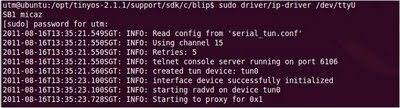
\includegraphics[scale=0.9]{img/tunnel_output.jpg}
\caption{IPv6 over USB tunnel execution output}
\label{fig:tunnel_output}
\end{figure}

\item To Run the Gateway Sensor Data TCP server do the following:
\subitem cd
\subitem cd grid-aui-tinyos/programming/GatewayServer/src
\subitem java Server

\item To Enable IP forwarding do the following:
\subitem sudo bash
\subitem echo 1 \textgreater /proc/sys/net/ipv4/ip\_forward
\subitem exit

\item  To drop all incoming packets: sudo iptables -P INPUT DROP
\item To disable ICPMP REDIRECT TO HOST:
\subitem sudo bash
\subitem /sbin/sysctl -w net.ipv4.conf.all.accept\_redirects=0
\subitem /sbin/sysctl -w net.ipv4.conf.all.send\_redirects=0
\subitem /sbin/sysctl -w net.ipv6.conf.all.accept\_redirects=0
\subitem /sbin/sysctl -w net.ipv6.conf.all.send\_redirects=0
\subitem exit

\item Run the Packet transformation process
\subitem cd
\subitem cd grid-aui-tinyos/programming/netfiltering
\subitem sudo my\_sniffer

\item Turn on the wireless sensor nodes one by one
\end{enumerate}

\paragraph{}
You should be able to get sensor data periodically. The mobile client access for turning On and Off will be explained in the Appendix C.

\end{document}